\documentclass[journal]{IEEEtran}

%\usepackage[retainorgcmds]{IEEEtrantools}
%\usepackage{bibentry}
\usepackage{xcolor,soul,framed} %,caption

\colorlet{shadecolor}{yellow}
% \usepackage{color,soul}
\usepackage[pdftex]{graphicx}
\graphicspath{{../pdf/}{../jpeg/}}
\DeclareGraphicsExtensions{.pdf,.jpeg,.png}

\usepackage[cmex10]{amsmath}
%Mathabx do not work on ScribTex => Removed
%\usepackage{mathabx}
\usepackage{array}
\usepackage{mdwmath}
\usepackage{mdwtab}
\usepackage{eqparbox}
\usepackage{url}


% ----------------------------------------------

% Definitions of languages: ------------
\usepackage{listings}
\lstdefinestyle{cStyle}{
  basicstyle=\scriptsize,
  breakatwhitespace=false,
  breaklines=true,
  captionpos=b,
  keepspaces=true,
  numbersep=5pt,
  showspaces=false,
  gobble=4,
  tabsize=4,
  showstringspaces=false,
  showtabs=false,
}
\renewcommand*{\lstlistingname}{Code}

% ----------------------------------------------




% \hyphenation{op-tical net-works semi-conduc-tor}

%\bstctlcite{IEEE:BSTcontrol}


%=== TITLE & AUTHORS ====================================================================
\begin{document}
\bstctlcite{IEEEexample:BSTcontrol}
    \title{YOLO Convolutional Neural Network}
  \author{Carlos~Matheus~Barros~da~Silva,~\IEEEmembership{Computer Engineering Bachelor Student of ITA}\\Prof. Marcos~Ricardo~Omena~de~Albuquerque~Máximo}

% The paper headers
\markboth{INSTITUTO TECNOLÓGICO DE AERONÁUTICA, May~2019
}{Neural Networks}

% ====================================================================
\maketitle


% === ABSTRACT ==============================================================
% ============================================================================
\begin{abstract}

This paper evaluates a Convolutional Neural Network known as YOLO (You Only Look Once), a very good Neural Network (NN) for computer vision.

In order to evaluate it, it was used a data set of robot socker in order to the NN identify the ball and the crossbars on the field.

It was observed that the YOLO NN worked as expected. The preditions to the posiotion of the objects were accurate.

% === KEYWORDS ===============================================================
% ============================================================================
\begin{IEEEkeywords}
    Keras, Neural Network, Convolutional Neural Network, YOLO
\end{IEEEkeywords}
\end{abstract}

\IEEEpeerreviewmaketitle

% ====================================================================
% ====================================================================
% ====================================================================


% === I. INTRODUCTION ========================================================
% =============================================================================
\section{Introduction}

\IEEEPARstart{N}{e}ural networks (NN) are computing systems vaguely inspired by the biological neural networks and astrocytes that constitute animal brains. The neural network itself is not an algorithm, but rather a framework for many different machine learning algorithms to work together and process complex data inputs. Such systems "learn" to perform tasks by considering examples, generally without being programmed with any task-specific rules. For example, an image recognition, they might learn to identify images that contain cats by analyzing example images that have been manually labeled as "cat" or "no cat" and using the results to identify cats in other images. They do this without any prior knowledge about cats, for example, that they have fur, tails, whiskers and cat-like faces. Instead, they automatically generate identifying characteristics from the learning material that they process.

Keras is an open-source neural-network library written in Python. It is capable of running on top of TensorFlow, Microsoft Cognitive Toolkit, Theano, or PlaidML. Designed to enable fast experimentation with deep neural networks, it focuses on being user-friendly, modular, and extensible. It was developed as part of the research effort of project ONEIROS (Open-ended Neuro-Electronic Intelligent Robot Operating System), and its primary author and maintainer is François Chollet, a Google engineer. Chollet also is the author of the XCeption deep neural network model.

In deep learning, a convolutional neural network (CNN, or ConvNet) is a class of deep neural networks, most commonly applied to analyzing visual imagery.

CNNs are regularized versions of multilayer perceptrons. Multilayer perceptrons usually refer to fully connected networks, that is, each neuron in one layer is connected to all neurons in the next layer. The "fully-connectedness" of these networks make them prone to overfitting data. Typical ways of regularization includes adding some form of magnitude measurement of weights to the loss function. However, CNNs take a different approach towards regularization: they take advantage of the hierarchical pattern in data and assemble more complex patterns using smaller and simpler patterns. Therefore, on the scale of connectedness and complexity, CNNs are on the lower extreme.

They are also known as shift invariant or space invariant artificial neural networks (SIANN), based on their shared-weights architecture and translation invariance characteristics.

% ==========================================================================
\section{Neural Network Implementation}

The implementation was based on the file \textit{yolo detector} and the file \textit{make detector network}. The first one is where the logic of getting the image, treat the image, pass it to the NN, and treat the result lies. While the second is where the Neural Network is defined.

The code of \textit{make detector network} can be seen in the Code \ref{code:nn} and the code of \textit{yolo detector} can be seen in the Code \ref{code:detector}.

\lstinputlisting[
    language=python,
    caption={Definition of the Neural Network with Keras},
    label={code:nn},
    style=cStyle,
    firstline=13,
    lastline=83
]{./../code/make_detector_network.py}

\lstinputlisting[
    language=python,
    caption={Logic to detect crossbars and ball using the NN},
    label={code:detector},
    style=cStyle,
    firstline=7,
    lastline=102
]{./../code/yolo_detector.py}

%-----------------------------------------------------------------------------
\section{Neural Network Analysis}
%-----------------------------------------------------------------------------
\subsection{YOLO Neural Network creation analysis}

Runing the file \textit{make detector network}, it is printed the NN defined in the code \ref{code:nn}. The details of the Neral Network can be seen on the file \ref{code:details}. It is possible to see that it is very similar to the proposed.

\lstinputlisting[
    language=python,
    caption={Details of the NN created with Keras},
    label={code:details},
    style=cStyle,
]{./../code/neural_network_details.txt}

%-----------------------------------------------------------------------------
\subsection{YOLO performance analysis}

In order to evaluate the YOLO Neural Network, it was used a model already trained to identify the ball and the crossbars in the socker field.

The YOLO performed very weel on the 10 cases having a 100\% acuracy. On the figures from Image \ref{} to Image \ref{} it is possible its identification in some test cases.

\begin{figure}
  \begin{center}
  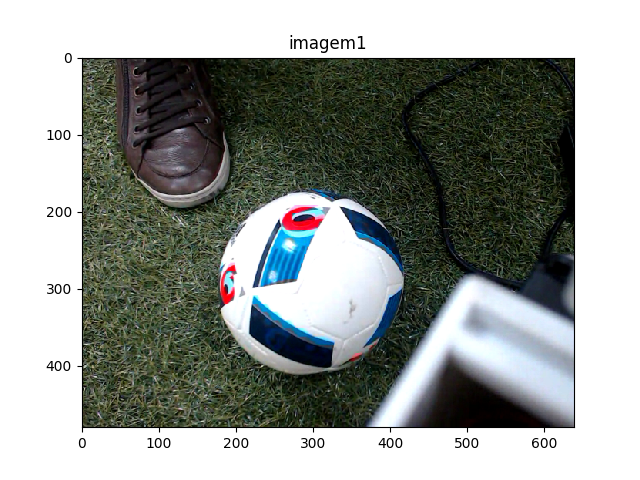
\includegraphics[width=2.8in]{./../code/imagem1_detection.png}
  \caption{Example of identification of ball and crossbars by the YOLO.}
  \label{img:classification_one}
  \end{center}
\end{figure}

\begin{figure}
  \begin{center}
  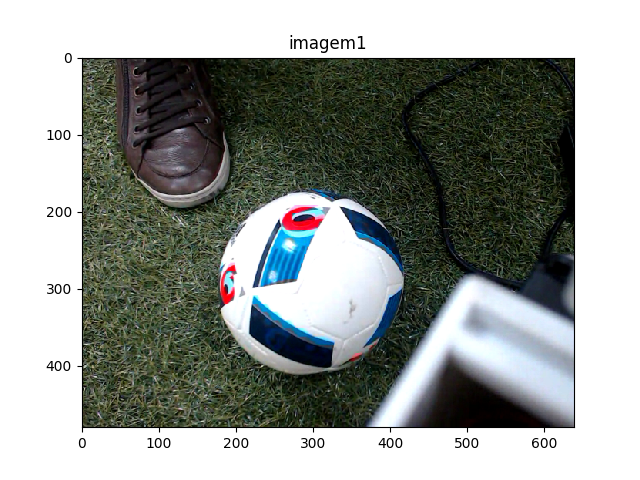
\includegraphics[width=2.8in]{./../code/imagem1_detection.png}
  \caption{Example of identification of ball and crossbars by the YOLO.}
  \label{img:classification_one}
  \end{center}
\end{figure}

\begin{figure}
  \begin{center}
  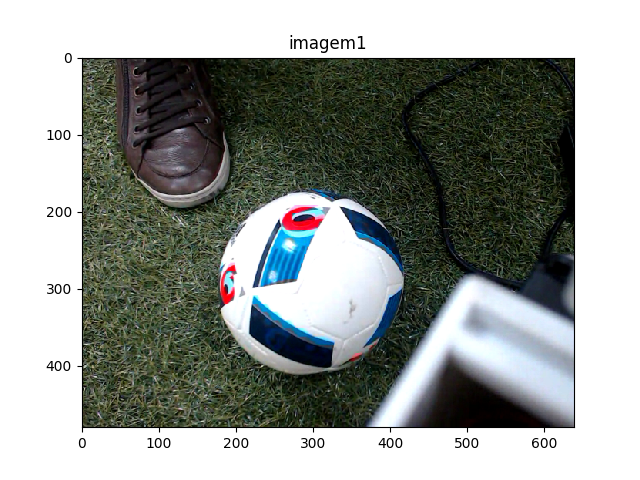
\includegraphics[width=2.8in]{./../code/imagem1_detection.png}
  \caption{Example of identification of ball and crossbars by the YOLO.}
  \label{img:classification_one}
  \end{center}
\end{figure}

\begin{figure}
  \begin{center}
  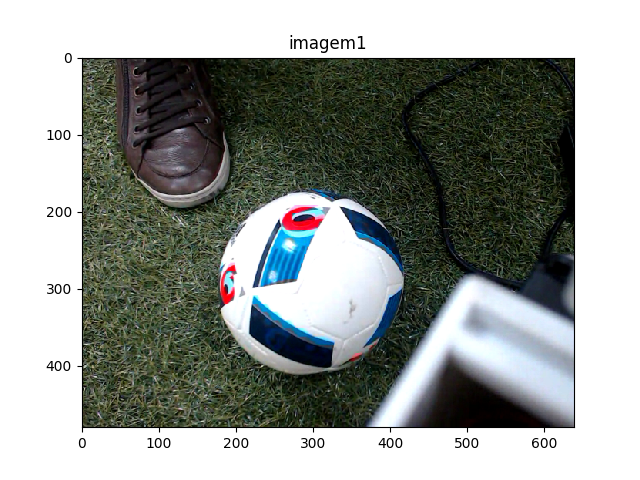
\includegraphics[width=2.8in]{./../code/imagem1_detection.png}
  \caption{Example of identification of ball and crossbars by the YOLO.}
  \label{img:classification_one}
  \end{center}
\end{figure}

\begin{figure}
  \begin{center}
  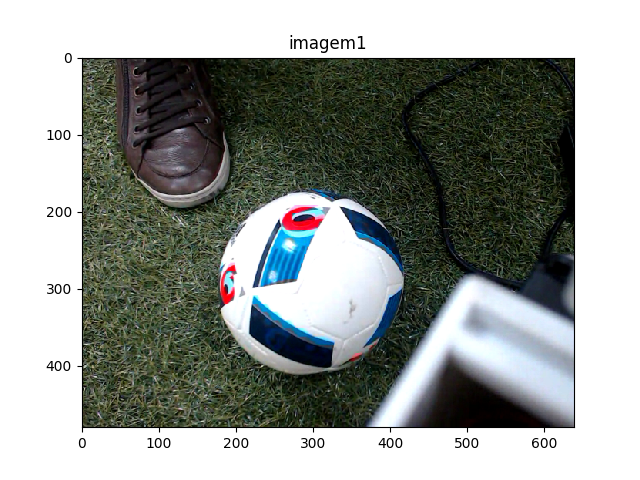
\includegraphics[width=2.8in]{./../code/imagem1_detection.png}
  \caption{Example of identification of ball and crossbars by the YOLO.}
  \label{img:classification_one}
  \end{center}
\end{figure}




As said before, in 1.3\% of the test cases ware misclassified. In Image \ref{img:misclassification_one} and Image \ref{img:misclassification_two} is possible to see two examples of test cases of misclassification.

\begin{figure}
  \begin{center}
  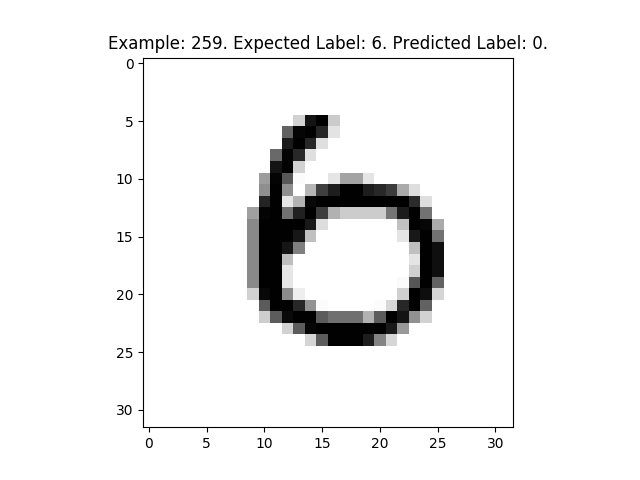
\includegraphics[width=2.8in]{./../code/misclassified_image_259.png}
  \caption{Example of a misclassified test case, was expected 6 and was predicted as 0.}
  \label{img:misclassification_one}
  \end{center}
\end{figure}

\begin{figure}
  \begin{center}
  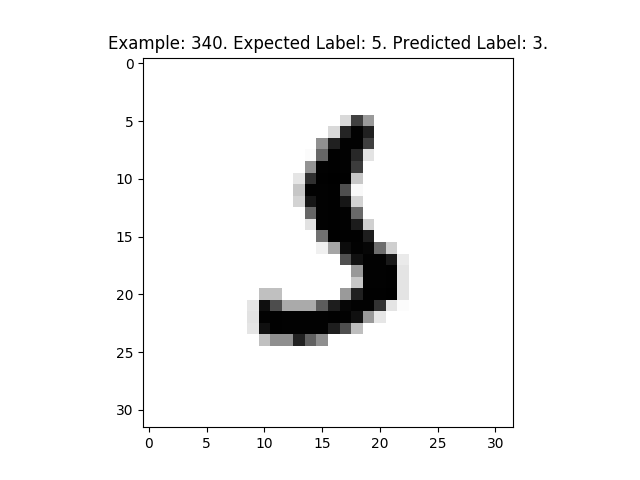
\includegraphics[width=2.8in]{./../code/misclassified_image_340.png}
  \caption{Example of a misclassified test case, was expected 5 and was predicted as 3.}
  \label{img:misclassification_two}
  \end{center}
\end{figure}

\subsection{LeNet-5 Convolutional Neural Network Analysis on TensorBoard}

In \textit{Tensor Board} it was possible to see that occured a fast decrase on loss function and a rapidly accuracy to converge in more than 98\% of acuracy. On Image \ref{img:accuracy} and Image \ref{img:loss_func} it is possible to see the graphs representing the converge of \textit{accuracy} and \textit{loss function} respectively.

\begin{figure}
  \begin{center}
  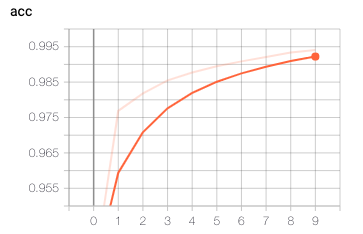
\includegraphics[width=2.8in]{./../code/tensorboard/tensor_board_accuracy_graph.png}
  \caption{Accuracy Graph generated by TensorBoard}
  \label{img:accuracy}
  \end{center}
\end{figure}

\begin{figure}
  \begin{center}
  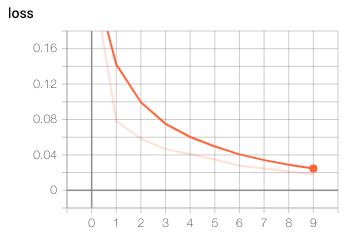
\includegraphics[width=2.8in]{./../code/tensorboard/tensor_board_loss_graph.png}
  \caption{Loss Function Graph generated by TensorBoard}
  \label{img:loss_func}
  \end{center}
\end{figure}

TensorBoard also provided an overview of the Neural Network format, this is denoted on Image \ref{img:tensorboard_main} and Image \ref{img:tensorboard_aux}.

\begin{figure}
  \begin{center}
  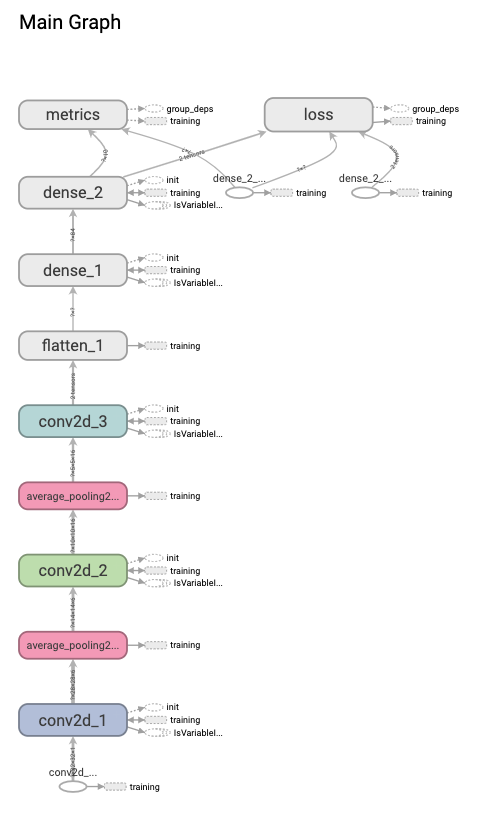
\includegraphics[width=2.8in]{./../code/tensorboard/tensor_board_main_graph.png}
  \caption{TensorBoard Main Graph.}
  \label{img:tensorboard_main}
  \end{center}
\end{figure}

\begin{figure}
  \begin{center}
  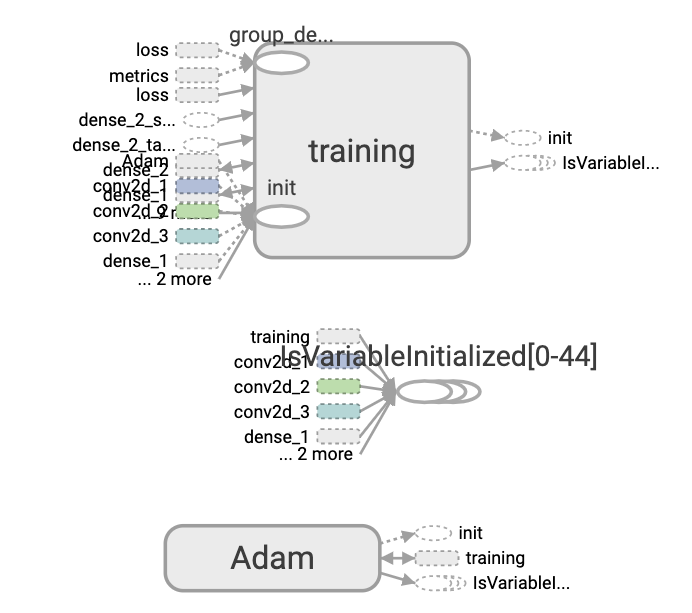
\includegraphics[width=2.8in]{./../code/tensorboard/tensor_board_auxiliary_nodes.png}
  \caption{TensorBoard Auxiliary Nodes.}
  \label{img:tensorboard_aux}
  \end{center}
\end{figure}

\section {Conclusion}

It was clear, therefore, that the Convolutional Neural Network worked as expected. The number prediction was very accurate having 98.7\% of accuracy on the data set.

\vfill
\end{document}
